\chapter{CGI Scripts}

\index{CGI}CGI scripts are programs that read input forms and generate
dynamic HTML content for the World Wide
Web. CGI programs are often written in \index{scripting languages}scripting
languages, but they can be written in any language, such as C.
Unicon is ideal for writing CGI scripts, since it
has extraordinary support for string processing. In this chapter you
will learn how to

\begin{itemize}
\item Construct programs whose input comes from a web server.
\item Process user input obtained from fields in HTML forms
\item Generate HTML output from your Icon programs
\end{itemize}

\section{Introduction to CGI}

The Common Gateway Interface, or CGI, defines the means by which Web
servers interact with external programs that assist in processing Web
input and output. CGI scripts are programs that are invoked by a Web
server to process input data from a user, or provide users with pages
of dynamically generated content, as opposed to static content found in
\index{HTML}HTML files. The primary
\index{reference!documentation}reference documentation on CGI is
available on the Web from the National Center for Supercomputer
Applications (NCSA) at \texttt{http://hoohoo.ncsa.uiuc.edu/cgi/}. If
you need a gentler treatment than the official reference, \textit{The
CGI Book}, by Bill Weinman, is a good book on CGI. Although other
methods for writing web applications on the server have been developed,
CGI is the most general, portable method and is likely to remain in
wide use for some time.

This chapter describes \texttt{cgi.icn}, a library of procedures for
writing CGI scripts. The \texttt{cgi.icn} library consists of a number
of procedures to simplify CGI input processing and especially the
generation of HTML-tagged output from various data structures. The
\texttt{cgi.icn} reference documentation can be found in Appendix B,
which describes many important modules in the Icon Program Library.

{\sffamily\bfseries Note}

{\sffamily To use \texttt{cgi.icn}, place the statement \texttt{link cgi}
at the top of your program.}

CGI programs use the hypertext markup language HTML as their output
format for communicating with the user through a Web browser.
Consequently, this chapter assumes you can cope with HTML, which is
beyond the scope of this book. HTML is an ASCII format that mixes plain
text with \textit{tags} consisting of names enclosed in angle brackets
such as \texttt{{\textless}HTML{\textgreater}}. HTML defines many tags.
A few common tags will be defined where they occur in the examples.
Most tags occur in pairs that mark the beginning and end of some
structure in the document. End tags have a slash character preceding
the name, as in \texttt{{\textless}/FONT{\textgreater}}. More details
on HTML are available from the World Wide Web Consortium at
\texttt{http://www.w3.org/MarkUp/}.

\subsection*{Organization of a CGI script}

CGI programs are very simple. They process input data supplied by the
Web browser that invoked the script (if any), and then write a new Web
page, in HTML, to their standard output. When you use \texttt{cgi.icn}
the input-processing phase is automatically completed before control is
passed to your program, which is organized around the HTML code that
you generate in response to the user. In fact, cgi.icn includes a
\texttt{main()} procedure that processes the input and writes HTML
header and tail information around your program's
output. For this reason,
when you use \texttt{cgi.icn}, you must call your main procedure
\texttt{cgimain()}.

\subsection*{Processing input}

The \index{HTTP}HTTP protocol includes two ways to invoke a CGI program,
with different methods of supplying user input, either from the
standard input or from a \texttt{QUERY\_STRING} environment variable.
In either case, the input is organized as a set of fields that were
given names in the HTML code from which the CGI program was invoked.
For example, an HTML form might include a tag such as: 

\iconcode{
\>   {\textless}INPUT TYPE = "text" NAME =
"PHONE" SIZE=15{\textgreater}}

\noindent
which allows input of a string of length up to 15 characters into a
field named \texttt{PHONE}.

After the CGI library processes the input, it provides applications with
the various fields from the input form in a single table, which is a
global variable named \texttt{cgi}. The keys of this table are exactly
the names given in the HTML \texttt{INPUT} tags. The values accessed
from the keys are the string values supplied by the user. For example,
to access the \texttt{PHONE} field from the above example, the
application could write 

\iconcode{
\>   cgi["PHONE"]}

\subsection*{Processing output}

The main task of the CGI program is to write an HTML page to its
standard output, and for this task \texttt{cgi.icn} provides a host of
procedures. Typically these procedures convert a structure value into a
string, wrapped with an appropriate HTML tag to format it properly. A
typical example is the library procedure
\texttt{cgiSelect(name,values)}, which writes an HTML \texttt{SELECT}
tag for a field named name. The \texttt{SELECT} tag creates a list of
radio buttons on an HTML form whose labels are given by a list of
strings in the second parameter to \texttt{cgiSelect()}. A programmer
might write

\iconcode{
\>   cgiSelect("GENDER",
["female",
"male"])}

\noindent to generate the HTML

\iconcode{
{\textless}SELECT
NAME="GENDER"{\textgreater} \\
{\textless}OPTION SELECTED{\textgreater}female \\
{\textless}OPTION{\textgreater}male \\
{\textless}/SELECT{\textgreater}
}

\subsection*{Common CGI environment variables}

The official CGI definition includes a set
of standard \index{environment variable!CGI standard}environment
variables that are set by the Web server as a method of passing
information to the CGI script. Programmers access these environment
variables using \texttt{getenv()}, as in

\iconcode{
\>   getenv("REMOTE\_HOST")}

Table 14-1 presents a summary of the CGI environment variables as a
convenience so that this book can serve as a stand-alone reference for
writing most CGI scripts. For a complete listing of all the environment
variables supported by CGI go to
\url{http://hoohoo.ncsa.uiuc.edu/cgi/env.html} on the Internet.

{\centering\sffamily\bfseries Table 14-1}

{\centering\sffamily\bfseries CGI Environment Variables}

\begin{flushleft}
\tablehead{}
\begin{xtabular}{|m{1.65in}|m{4.15in}|}
\hline
\sffamily\bfseries Variable &
\sffamily\bfseries Explanation\\\hline
\texttt{CONTENT\_LENGTH} &
The length of the ASCII string provided by
\texttt{method="POST"}.\\\hline
\texttt{HTTP\_USER\_AGENT} &
The user's browser software and proxy gateway, if any.
The format is \texttt{\textit{name/version}}, but varies
wildly.\\\hline
\texttt{QUERY\_STRING} &
The information submitted through the form, which follows the ? in the
URL when using \texttt{method="GET"}.
\texttt{QUERY\_STRING} data is parsed and inserted into a table
stored in the global variable \texttt{cgi}, so
\texttt{cgi.icn} scripts do not generally consult this environment
variable.\\\hline
\texttt{REMOTE\_ADDR} &
The IP address of the client machine.\\\hline
\texttt{REMOTE\_HOST} &
The hostname of the client machine. Defaults to IP held by
\texttt{REMOTE\_ADDR}.\\\hline
\texttt{REQUEST\_METHOD} &
The method (\texttt{GET} or \texttt{POST)} used to invoke the CGI
script.\\\hline
\texttt{SERVER\_NAME} &
The server's hostname. It defaults to the IP
address.\\\hline
\texttt{SERVER\_SOFTWARE} &
The Web server that invoked the CGI script. The format is
\texttt{\textit{name/version}}.\\\hline
\end{xtabular}
\end{flushleft}

\section{The CGI Execution Environment}

CGI scripts do not execute as stand-alone programs and
aren't launched from a command line; a Web server
executes them. The details of this are necessarily dependent on the
operating system and Web server combination in use. The following
examples are based on a typical UNIX Apache server installation in
which users' HTML files are located under
\texttt{\$HOME/public\_html}. Check with your system administrator or
Web server documentation for the specific filenames, directories, and
permissions required to execute scripts from your Web server. Some web
servers do not allow scripts at all, and most others run scripts with a
special userid in a limited/protected file system where absolute
pathnames are different from how you see them.

Under Apache, you need a directory under
\texttt{\$HOME/public\_html} named \texttt{cgi-bin}. Both
\texttt{\$HOME/public\_html} and its \texttt{cgi-bin} subdirectory
should have "group" and
"other" permissions set to allow
reading and executing for the Web server to run the programs you place
there. Do not give anyone but yourself write permissions! The following
commands set things up on a typical Apache system. The percent sign
(\texttt{\%}) is not part of the command; it is the UNIX shell prompt.
The period in the final command is part of the command and refers to
the current working directory.

\iconcode{
\% mkdir \$HOME/public\_html \\
\% cd \$HOME/public\_html \\
\% mkdir cgi-bin \\
\% chmod go+rx . cgi-bin
}

The next two example files will allow you to verify that your
directories and permissions are correct for your Web server.
Despite all the attempts to make the world's web servers secure,
the only security you can count on is your own. From security expert
David A. Gamey we have the following tips:

\newenvironment{itemize*}%
  {\begin{itemize}%
    \setlength{\itemsep}{0pt}%
    \setlength{\parskip}{0pt}}%
  {\end{itemize}}
\begin{itemize*}
\item Use no data without checking for validity. Even HTTP header data
can be wrong. If you expect a number, make sure the supplied data
is a number.
\item It is a very bad idea to make any \texttt{system()} calls (or open
piped commands, etc.) from scripts. If you absolutely have to run something
external, construct command strings yourself or fully parse user data being
used to check for command separators and hidden commands, etc.
\item Don't rely on looking for known bad characters; restrict input to
known good characters. Use known good values such as those selected from
list boxes
\item Sensitive data should be sent using POST, not GET.
\item Check for and prevent file system attacks, such as
paths including .. in them.
\item Log everything received by your script, so you can
tell when attacks occur.
\end{itemize*}

\section{An Example HTML Form}

CGI scripts are typically invoked from HTML pages.
When you view the following example page in your browser,
it should look something like the one shown in Figure 14-1.
For this test, create an HTML form \texttt{\$HOME/public\_html/simple.html}
containing Listing 14-1. When you have a CGI script compiled and ready to
run, you can edit the URL in this file to point at your CGI program, the
\texttt{simple.cgi} executable.
\begin{center}
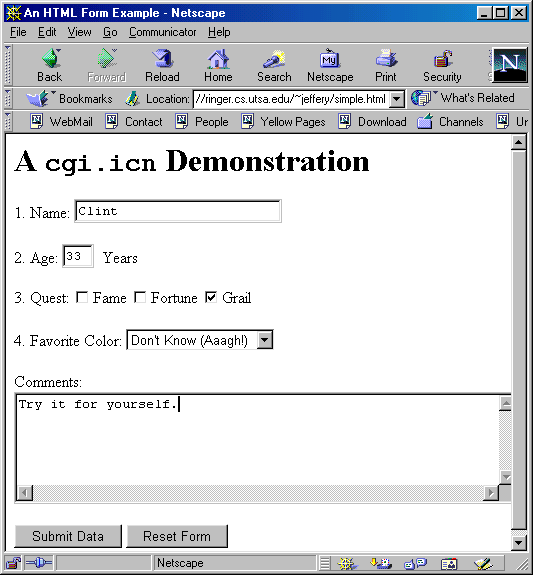
\includegraphics[width=4.05in,height=4.36in]{ub-img/ub-img44.png}
\end{center}
{\sffamily\bfseries Figure 14-1:}
{\sffamily An HTML Form Example}


{\sffamily\bfseries Listing 14-1}
{\sffamily\bfseries An HTML form}

\iconcode{
{\textless}HTML{\textgreater}{\textless}HEAD{\textgreater}{\textless}title{\textgreater}
An HTML Form Example
{\textless}/title{\textgreater}{\textless}/HEAD{\textgreater} \\
{\textless}BODY{\textgreater} \\
{\textless}h1{\textgreater} A
{\textless}tt{\textgreater}cgi.icn{\textless}/tt{\textgreater}
Demonstration{\textless}/h1{\textgreater} \\
{\textless}form method="GET" \\
\>   \ \
action="http://www.cs.uidaho.edu/\~{}jeffery/cgi-bin/simple.cgi"{\textgreater} \\
1. Name: {\textless}input type="text"
name="name" size=25{\textgreater}
{\textless}p{\textgreater} \\
2. Age: \ {\textless}input type="text"
name="age" size=3{\textgreater}
\&nbsp;Years {\textless}p{\textgreater} \\
3. Quest: \\
{\textless}input type="checkbox"
name="fame"{\textgreater}Fame{\textless}/input{\textgreater} \\
{\textless}input type="checkbox"
name="fortune"{\textgreater}Fortune{\textless}/input{\textgreater} \\
{\textless}input type="checkbox"
name="grail"{\textgreater}Grail{\textless}/input{\textgreater}{\textless}p{\textgreater} \\
4. Favorite Color: \\
{\textless}select
name="color"{\textgreater} \\
{\textless}option{\textgreater}Red \\
{\textless}option{\textgreater}Green \\
{\textless}option{\textgreater}Blue \\
{\textless}option selected{\textgreater}Don't Know
(Aaagh!) \\
{\textless}/select{\textgreater}{\textless}p{\textgreater} \\
Comments:{\textless}br{\textgreater} \\
{\textless}textarea rows=5 cols=60
name="comments"{\textgreater}{\textless}/textarea{\textgreater}{\textless}p{\textgreater} \\
{\textless}input type="submit"
value="Submit Data"{\textgreater} \\
{\textless}input type="reset"
value="Reset Form"{\textgreater} \\
{\textless}/form{\textgreater} \\
{\textless}/BODY{\textgreater} \\
{\textless}/HTML{\textgreater}
}


\section{An Example CGI Script: Echoing the User's Input}

The following script, named \texttt{simple.cgi} might be invoked from
the \texttt{FORM} tag above. The \texttt{simple.cgi} script is produced
from an Unicon source file, \texttt{simple.icn}\texttt{,} that you can
copy from the book web site
(\texttt{http://unicon.org/book/}). This program needs to
be compiled with the command

\iconcode{
unicon \textrm{$-$}o simple.cgi simple.icn }

Many Web servers are configured so that CGI scripts must end with the
extension \texttt{.cgi}. Check with your system administrator about CGI
naming conventions if the \texttt{.cgi} extension does not work for
you. In addition to the web server being configured to allow user
invocation, unless you use compiler option \texttt{{}-B} to bundle the
virtual machine into your executable, your program must be able to find
and execute the virtual machine from whatever user id
CGI's are executed.

The program reads the form input specified in \texttt{simple.html}, and
writes it back out. All \texttt{cgiEcho()} is doing in this case is
adding an HTML newline tag after each call. If you look it up in
Appendix B, you will find that it will copy its arguments to both the
HTML output and a log file if given a file as its first argument.

\iconcode{
link cgi \\
procedure cgimain() \\
\>   cgiEcho("Hello, ",
cgi["name"],
"!") \\
\>   cgiEcho("Are you really ", cgi["age"], " years old?") \\
\>   cgiEcho("You seek: ", cgi["fame"]==="on" \& "fame") \\
\>   cgiEcho("You seek: ", cgi["fortune"]==="on" \& "fortune") \\
\>   cgiEcho("You seek: ", cgi["grail"]==="on" \& "grail") \\
\>   cgiEcho("Your favorite color is: ", cgi["color"]) \\
\>   cgiEcho("Your comments: ",
cgi["comments"]) \\
end
}

Generating an output page that rehashes the user's
input is a good test of your HTML form before you deploy it with a CGI
script that actually does something. In some cases, it is also helpful
in allowing the user to recheck their submitted input and confirm or
cancel before acting on it.

\section{Debugging CGI Programs}

CGI programs can be a pain to debug. You may have to debug your CGI
execution environment, before you can even start debugging your CGI
program itself. If your CGI script returns an "internal
server error", or no output at all, you may have file
permissions wrong, or the CGI script may not be able to find the Unicon
virtual machine in order to run the program. Some web servers execute
CGI scripts under a special userid such as
"web", others will run them under your user
id. Some web servers run CGI scripts under a protected file system
where the root directory "/" is not the
same as the root directory visible to your user account, so the path to
iconx that you normally use may be invalid in your CGI program. CGI
scripts may have a very limited PATH for security reasons, not the PATH
you set for your user account. \ Your best bet is probably to use the
-B Unicon compiler option to bundle the Unicon interpreter into your
executable file; alternatively you can probably copy the virtual
machine "iconx" into your cgi-bin directory

Debugging your CGI program itself may require special tricks. Because
your CGI program is executed by a web server, its standard error output
may not be visible to you. \ You can try to redirect error output to
standard out, but your error output may not be readable unless it is
converted into HTML (say, by adding
\texttt{{\textless}BR{\textgreater}} at each newline). One way to
accomplish this is to write \textit{two} programs: one that performs
the primary task, and a second program that calls the first one,
catches any error messages, and converts any plain text output to HTML.

\section{Appform: An Online Scholarship Application}

The next example, \texttt{appform.icn}, is a CGI script for an
on-line scholarship application that was used at a university. Its
structure is similar to the previous example, with a twist:
the user input is printed for the convenience of the scholarship
administrators. As a backup, the CGI script also e-mails the
application to the scholarship administrator. This is useful if the
print job fails for some reason.
The program is a single \texttt{cgimain()} procedure, which starts by
processing each of the user input fields. The program then opens a
temporary file with a \texttt{.txt} extension, and writes a nicely
formatted document containing the user's scholarship
application information.

The code for Appform is shown in Listing 14-2. To run it you must
adapt it to your environment. As written, it prints to
\texttt{lpr}, and sends mail to \texttt{jeffery@cs.uidaho.edu}. When running a
CGI script it is important to realize you will run in a different
directory, and with different user id and PATH environment, than your
regular account. The program runs with whatever user id and
permissions the system administrator assigns the Web server
process. For example, its root (/) directory may not be at the root of
your regular filesystem, so absolute paths may not work.

{\sffamily\bfseries
Listing 14-2}

{\sffamily\bfseries
An online application form}

\iconcode{
\#\#\#\#\#\#\#\#\#\#\#\#\#\#\#\#\#\#\#\#\#\#\#\#\#\#\#\#\#\#\#\#\#\#\#\#\#\#\#\#\#\#\#\#\#\#\#\#\#\#\#\#\#\#\#\#\#\#\#\#\#\#
 \\
\# \ \ \ \ \ \ File: \ \ \ appform.icn \\
\# \ \ \ \ \ \ Subject: CGI program to process scholarship applications \\
\# \ \ \ \ \ \ Author: \ Clinton Jeffery \\
\# \ \ \ \ \ \ Date: \ \ \ July 11, 2002 \\
\#\#\#\#\#\#\#\#\#\#\#\#\#\#\#\#\#\#\#\#\#\#\#\#\#\#\#\#\#\#\#\#\#\#\#\#\#\#\#\#\#\#\#\#\#\#\#\#\#\#\#\#\#\#\#\#\#\#\#\#\#\#
 \\
\# This program processes a bunch of input fields defined in an
on-line schol-\\
\# arship application at http://unicon.org/book/appform.html and from them,\\
\# generates a text file, prints and e-mails it to the scholarship coordinator. \\
\#\#\#\#\#\#\#\#\#\#\#\#\#\#\#\#\#\#\#\#\#\#\#\#\#\#\#\#\#\#\#\#\#\#\#\#\#\#\#\#\#\#\#\#\#\#\#\#\#\#\#\#\#\#\#\#\#\#\#\#\#\#
 \\
\ \\
link cgi, io \\
\$define ADMIN "jeffery@cs.uidaho.edu" \\
procedure cgimain() \\
\ \ fname := tempname("appform", ".txt", "/tmp") \\
\ \ f := open(fname, "w") {\textbar} stop("can't open ", fname) \\
\ \ write("Generating typeset copy of application
form...") \\
\ \ write(f,"Scholarship Program
Application{\textbackslash}n") \\
\ \ write(f, "Name: ",
cgi["NAME"],
"{\textbackslash}t{\textbackslash}t Phone: ", cgi["PHONE"]) \\
\ \ write(f, "Address: ", cgi["ADDRESS1"], '
{\textbackslash}t{\textbackslash}t Social Sec. Number: ", cgi["SOC"]) \\
\ \ write(f, cgi["ADDRESS2"],
" {\textbackslash}t{\textbackslash}t Gender (M/F):
",cgi["GENDER"],
"{\textbackslash}n") \\
\ \ write(f,"Semester hours completed: ",
cgi["CREDITS"]) \\
\ \ write(f,"College GPA: \ Overall ",
cgi["GPA"]) \\
\ \ write(f,"Present Employer: ",
cgi["EMPLOYER"]) \\
\ \ write(f,"Position: ", cgi["POSITION"], " Hours/week: ", cgi["HOURS"]) \\
\ \ write(f,"Educational Background") \\
\ \ write(f,"High School: name, year, GPA,
		graduated?") \\
\ \ write(f, cgi["HIGH1"],
"{\textbackslash}n",
cgi["HIGH2"]) \\
\ \ write(f,"For each college, list name, dates attended,
credit hours,") \\
\ \ write(f,"degrees awarded", cgi["COLL1"], "{\textbackslash}n", cgi["COLL2"],
"{\textbackslash}n{\textbackslash}n") \\
\ \ write(f,"Academic honors, scholarships, and
fellowships") \\
\ \ write(f,cgi["HONOR1"],
"{\textbackslash}n",
cgi["HONOR2"],
"{\textbackslash}n") \\
\ \ write(f,"Extracurricular interests:", cgi["EXTRA1"],
"{\textbackslash}n",
cgi["EXTRA2"]) \\
\ \ write(f,"Professional organizations:",
cgi["ORGS1"],
"{\textbackslash}n",
cgi["ORGS2"]) \\
\ \ write(f,"Research interests:") \\
\ \ write(f,cgi["RESEARCH1"],
"{\textbackslash}n",
cgi["RESEARCH2"]) \\
\ \ write(f,"Name(s) of at least one person you have asked
to") \\
\ \ write(f,"write an academic reference
letter.") \\
\ \ write(f,"Name \ \ \ \ \ \ \ \ \ \ \ Address
\ \ \ \ \ \ \ \ Relationship") \\
\ \ write(f,cgi["REF1"],
"{\textbackslash}t",
cgi["REFADD1"],
"{\textbackslash}t",cgi["REFREL1"]) \\
\ \ write(f,cgi["REF2"],
"{\textbackslash}t",
cgi["REFADD2"],
"{\textbackslash}t",cgi["REFREL2"]) \\
\ \ write(f,"{\textbackslash}nI certify that information
provided on this") \\
\ \ write(f,"application is correct and complete to my
knowledge.{\textbackslash}n") \\
\ \ write(f,"Signature: ",
repl("\_", 60), "{\textbackslash}n Date: ",
repl("\_", 60), 
"{\textbackslash}n{\textbackslash}\^{}l{\textbackslash}n") \\
\ \ write(f,"Please write a short statement of purpose,
including") \\
\ \ write(f,"information about your background, major, and
career") \\
\ \ write(f,"interests, and professional
goals.{\textbackslash}n") \\
\ \ write(f, cgi["INFO"]) \\
\ \ close(f) \\
\ \ write("Mailing form to program director...") \\
\ \ f := open(fname) \\
\ \ m := open("mailto:" {\textbar}{\textbar} ADMIN, "m", "Subject: appform") \\
\ \ while write(m, read(f)) \\
\ \ close(m) \\
\ \ close(f) \\
\ \ write("Printing hard copy...") \\
\ \ system("lpr " {\textbar}{\textbar} fname {\textbar}{\textbar} "; rm " {\textbar}{\textbar} fname) \\
\ \ cgiEcho("Thank you for applying, ",
cgi["NAME"]) \\
\ \ cgiEcho("Your application has been submitted to
" {\textbar}{\textbar} ADMIN) \\
end
}

\section*{Summary}

Writing CGI scripts in Unicon is easy. The input fields are handed to
you elegantly in a global variable, and library functions allow you to
write terse code that generates correct HTML output. The only thing
certain about the fast-changing Internet standards is that they will
get continually more complex at a rapid pace. CGI scripting is no
substitute for \index{JavaScript}JavaScript, \index{XML}XML, or any
newer buzzword that may be hot this week. But it is a lasting,
multi-platform standard for how to run a program on a Web server from a
browser, and it may be the simplest and best solution for many Internet
applications for some time.
